% author: Simon Bachmann
\section{Problem Statement}\label{sec:problem-statement}
Today's event ticketing industry has a fundamental flaw. The existing systems for distributing tickets are open for a lot of arbitrage during the time the ticket is sold until the event happens. This means that besides the primary seller of the tickets (e.g. event organizer) intermediaries make a profit by buying, reselling and counterfeiting tickets. 

Figure \ref{fig:ticketing-industry-landscape} gives an overview of today's event ticketing landscape with its most important actors and how they interact with each other. The secondary market is where the major issue lies and ticket scalpers can scoop profits through it.

\begin{figure}[H]
    \centering
    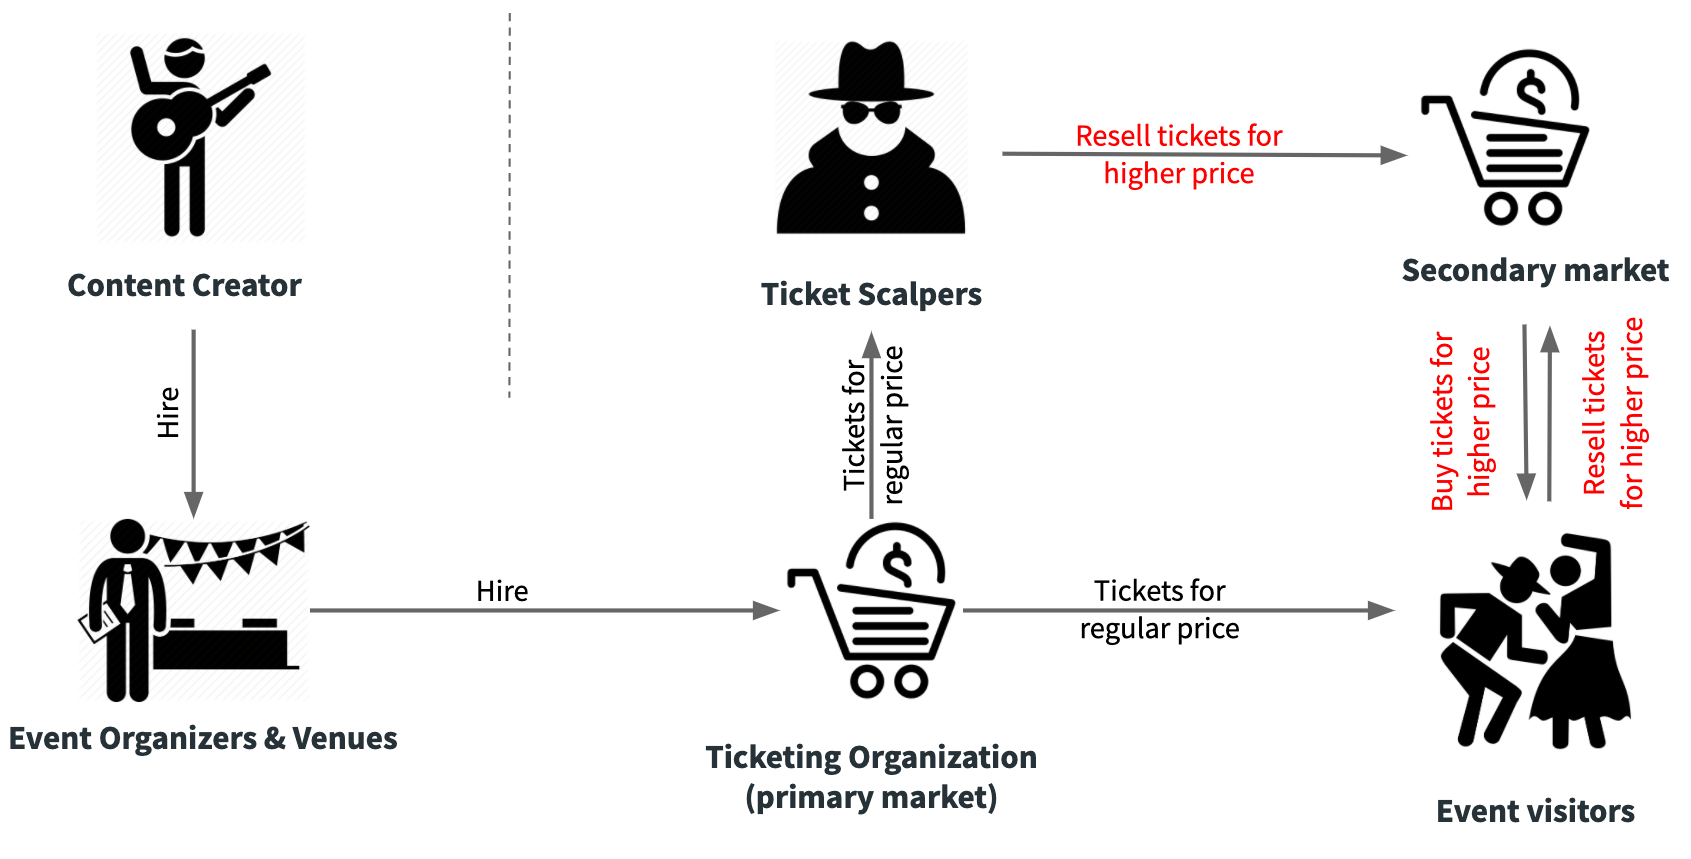
\includegraphics[width=16cm]{figures/ticketing-industry-landscape.png}
    \caption{Actors in the ticketing industry}
    \label{fig:ticketing-industry-landscape}
\end{figure}
